\documentclass[1p]{elsarticle_modified}
%\bibliographystyle{elsarticle-num}

%\usepackage[colorlinks]{hyperref}
%\usepackage{abbrmath_seonhwa} %\Abb, \Ascr, \Acal ,\Abf, \Afrak
\usepackage{amsfonts}
\usepackage{amssymb}
\usepackage{amsmath}
\usepackage{amsthm}
\usepackage{scalefnt}
\usepackage{amsbsy}
\usepackage{kotex}
\usepackage{caption}
\usepackage{subfig}
\usepackage{color}
\usepackage{graphicx}
\usepackage{xcolor} %% white, black, red, green, blue, cyan, magenta, yellow
\usepackage{float}
\usepackage{setspace}
\usepackage{hyperref}

\usepackage{tikz}
\usetikzlibrary{arrows}

\usepackage{multirow}
\usepackage{array} % fixed length table
\usepackage{hhline}

%%%%%%%%%%%%%%%%%%%%%
\makeatletter
\renewcommand*\env@matrix[1][\arraystretch]{%
	\edef\arraystretch{#1}%
	\hskip -\arraycolsep
	\let\@ifnextchar\new@ifnextchar
	\array{*\c@MaxMatrixCols c}}
\makeatother %https://tex.stackexchange.com/questions/14071/how-can-i-increase-the-line-spacing-in-a-matrix
%%%%%%%%%%%%%%%

\usepackage[normalem]{ulem}

\newcommand{\msout}[1]{\ifmmode\text{\sout{\ensuremath{#1}}}\else\sout{#1}\fi}
%SOURCE: \msout is \stkout macro in https://tex.stackexchange.com/questions/20609/strikeout-in-math-mode

\newcommand{\cancel}[1]{
	\ifmmode
	{\color{red}\msout{#1}}
	\else
	{\color{red}\sout{#1}}
	\fi
}

\newcommand{\add}[1]{
	{\color{blue}\uwave{#1}}
}

\newcommand{\replace}[2]{
	\ifmmode
	{\color{red}\msout{#1}}{\color{blue}\uwave{#2}}
	\else
	{\color{red}\sout{#1}}{\color{blue}\uwave{#2}}
	\fi
}

\newcommand{\Sol}{\mathcal{S}} %segment
\newcommand{\D}{D} %diagram
\newcommand{\A}{\mathcal{A}} %arc


%%%%%%%%%%%%%%%%%%%%%%%%%%%%%5 test

\def\sl{\operatorname{\textup{SL}}(2,\Cbb)}
\def\psl{\operatorname{\textup{PSL}}(2,\Cbb)}
\def\quan{\mkern 1mu \triangleright \mkern 1mu}

\theoremstyle{definition}
\newtheorem{thm}{Theorem}[section]
\newtheorem{prop}[thm]{Proposition}
\newtheorem{lem}[thm]{Lemma}
\newtheorem{ques}[thm]{Question}
\newtheorem{cor}[thm]{Corollary}
\newtheorem{defn}[thm]{Definition}
\newtheorem{exam}[thm]{Example}
\newtheorem{rmk}[thm]{Remark}
\newtheorem{alg}[thm]{Algorithm}

\newcommand{\I}{\sqrt{-1}}
\begin{document}

%\begin{frontmatter}
%
%\title{Boundary parabolic representations of knots up to 8 crossings}
%
%%% Group authors per affiliation:
%\author{Yunhi Cho} 
%\address{Department of Mathematics, University of Seoul, Seoul, Korea}
%\ead{yhcho@uos.ac.kr}
%
%
%\author{Seonhwa Kim} %\fnref{s_kim}}
%\address{Center for Geometry and Physics, Institute for Basic Science, Pohang, 37673, Korea}
%\ead{ryeona17@ibs.re.kr}
%
%\author{Hyuk Kim}
%\address{Department of Mathematical Sciences, Seoul National University, Seoul 08826, Korea}
%\ead{hyukkim@snu.ac.kr}
%
%\author{Seokbeom Yoon}
%\address{Department of Mathematical Sciences, Seoul National University, Seoul, 08826,  Korea}
%\ead{sbyoon15@snu.ac.kr}
%
%\begin{abstract}
%We find all boundary parabolic representation of knots up to 8 crossings.
%
%\end{abstract}
%\begin{keyword}
%    \MSC[2010] 57M25 
%\end{keyword}
%
%\end{frontmatter}

%\linenumbers
%\tableofcontents
%
\newcommand\colored[1]{\textcolor{white}{\rule[-0.35ex]{0.8em}{1.4ex}}\kern-0.8em\color{red} #1}%
%\newcommand\colored[1]{\textcolor{white}{ #1}\kern-2.17ex	\textcolor{white}{ #1}\kern-1.81ex	\textcolor{white}{ #1}\kern-2.15ex\color{red}#1	}

{\Large $\underline{12a_{0275}~(K12a_{0275})}$}

\setlength{\tabcolsep}{10pt}
\renewcommand{\arraystretch}{1.6}
\vspace{1cm}\begin{tabular}{m{100pt}>{\centering\arraybackslash}m{274pt}}
\multirow{5}{120pt}{
	\centering
	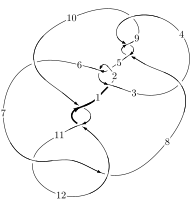
\includegraphics[width=112pt]{../../../GIT/diagram.site/Diagrams/png/1076_12a_0275.png}\\
\ \ \ A knot diagram\footnotemark}&
\allowdisplaybreaks
\textbf{Linearized knot diagam} \\
\cline{2-2}
 &
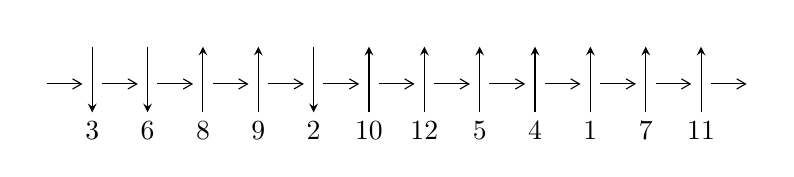
\begin{tikzpicture}[x=20pt, y=17pt]
	% nodes
	\node (C0) at (0, 0) {};
	\node (C1) at (1, 0) {};
	\node (C1U) at (1, +1) {};
	\node (C1D) at (1, -1) {3};

	\node (C2) at (2, 0) {};
	\node (C2U) at (2, +1) {};
	\node (C2D) at (2, -1) {6};

	\node (C3) at (3, 0) {};
	\node (C3U) at (3, +1) {};
	\node (C3D) at (3, -1) {8};

	\node (C4) at (4, 0) {};
	\node (C4U) at (4, +1) {};
	\node (C4D) at (4, -1) {9};

	\node (C5) at (5, 0) {};
	\node (C5U) at (5, +1) {};
	\node (C5D) at (5, -1) {2};

	\node (C6) at (6, 0) {};
	\node (C6U) at (6, +1) {};
	\node (C6D) at (6, -1) {10};

	\node (C7) at (7, 0) {};
	\node (C7U) at (7, +1) {};
	\node (C7D) at (7, -1) {12};

	\node (C8) at (8, 0) {};
	\node (C8U) at (8, +1) {};
	\node (C8D) at (8, -1) {5};

	\node (C9) at (9, 0) {};
	\node (C9U) at (9, +1) {};
	\node (C9D) at (9, -1) {4};

	\node (C10) at (10, 0) {};
	\node (C10U) at (10, +1) {};
	\node (C10D) at (10, -1) {1};

	\node (C11) at (11, 0) {};
	\node (C11U) at (11, +1) {};
	\node (C11D) at (11, -1) {7};

	\node (C12) at (12, 0) {};
	\node (C12U) at (12, +1) {};
	\node (C12D) at (12, -1) {11};
	\node (C13) at (13, 0) {};

	% arrows
	\draw[->,>={angle 60}]
	(C0) edge (C1) (C1) edge (C2) (C2) edge (C3) (C3) edge (C4) (C4) edge (C5) (C5) edge (C6) (C6) edge (C7) (C7) edge (C8) (C8) edge (C9) (C9) edge (C10) (C10) edge (C11) (C11) edge (C12) (C12) edge (C13) ;	\draw[->,>=stealth]
	(C1U) edge (C1D) (C2U) edge (C2D) (C3D) edge (C3U) (C4D) edge (C4U) (C5U) edge (C5D) (C6D) edge (C6U) (C7D) edge (C7U) (C8D) edge (C8U) (C9D) edge (C9U) (C10D) edge (C10U) (C11D) edge (C11U) (C12D) edge (C12U) ;
	\end{tikzpicture} \\
\hhline{~~} \\& 
\textbf{Solving Sequence} \\ \cline{2-2} 
 &
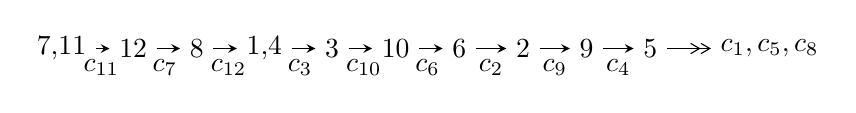
\begin{tikzpicture}[x=23pt, y=7pt]
	% node
	\node (A0) at (-1/8, 0) {7,11};
	\node (A1) at (1, 0) {12};
	\node (A2) at (2, 0) {8};
	\node (A3) at (49/16, 0) {1,4};
	\node (A4) at (33/8, 0) {3};
	\node (A5) at (41/8, 0) {10};
	\node (A6) at (49/8, 0) {6};
	\node (A7) at (57/8, 0) {2};
	\node (A8) at (65/8, 0) {9};
	\node (A9) at (73/8, 0) {5};
	\node (C1) at (1/2, -1) {$c_{11}$};
	\node (C2) at (3/2, -1) {$c_{7}$};
	\node (C3) at (5/2, -1) {$c_{12}$};
	\node (C4) at (29/8, -1) {$c_{3}$};
	\node (C5) at (37/8, -1) {$c_{10}$};
	\node (C6) at (45/8, -1) {$c_{6}$};
	\node (C7) at (53/8, -1) {$c_{2}$};
	\node (C8) at (61/8, -1) {$c_{9}$};
	\node (C9) at (69/8, -1) {$c_{4}$};
	\node (A10) at (11, 0) {$c_{1},c_{5},c_{8}$};

	% edge
	\draw[->,>=stealth]	
	(A0) edge (A1) (A1) edge (A2) (A2) edge (A3) (A3) edge (A4) (A4) edge (A5) (A5) edge (A6) (A6) edge (A7) (A7) edge (A8) (A8) edge (A9) ;
	\draw[->>,>={angle 60}]	
	(A9) edge (A10);
\end{tikzpicture} \\ 

\end{tabular} \\

\footnotetext{
The image of knot diagram is generated by the software ``\textbf{Draw programme}" developed by Andrew Bartholomew(\url{http://www.layer8.co.uk/maths/draw/index.htm\#Running-draw}), where we modified some parts for our purpose(\url{https://github.com/CATsTAILs/LinksPainter}).
}\phantom \\ \newline 
\centering \textbf{Ideals for irreducible components\footnotemark of $X_{\text{par}}$} 
 
\begin{align*}
I^u_{1}&=\langle 
2.60711\times10^{31} u^{97}+4.13570\times10^{31} u^{96}+\cdots+1.17609\times10^{31} b-9.51207\times10^{31},\\
\phantom{I^u_{1}}&\phantom{= \langle  }7.27315\times10^{30} u^{97}+3.06066\times10^{31} u^{96}+\cdots+1.76413\times10^{31} a-1.12339\times10^{32},\;u^{98}+2 u^{97}+\cdots-11 u-3\rangle \\
I^u_{2}&=\langle 
-2 u^2 b+b^2+u^2-3 u+1,\;- u^2+a+u,\;u^3- u^2+1\rangle \\
I^u_{3}&=\langle 
- u^2+b,\;- u^2+a- u,\;u^3+u^2-1\rangle \\
\\
\end{align*}
\raggedright * 3 irreducible components of $\dim_{\mathbb{C}}=0$, with total 107 representations.\\
\footnotetext{All coefficients of polynomials are rational numbers. But the coefficients are sometimes approximated in decimal forms when there is not enough margin.}
\newpage
\renewcommand{\arraystretch}{1}
\centering \section*{I. $I^u_{1}= \langle 2.61\times10^{31} u^{97}+4.14\times10^{31} u^{96}+\cdots+1.18\times10^{31} b-9.51\times10^{31},\;7.27\times10^{30} u^{97}+3.06\times10^{31} u^{96}+\cdots+1.76\times10^{31} a-1.12\times10^{32},\;u^{98}+2 u^{97}+\cdots-11 u-3 \rangle$}
\flushleft \textbf{(i) Arc colorings}\\
\begin{tabular}{m{7pt} m{180pt} m{7pt} m{180pt} }
\flushright $a_{7}=$&$\begin{pmatrix}0\\u\end{pmatrix}$ \\
\flushright $a_{11}=$&$\begin{pmatrix}1\\0\end{pmatrix}$ \\
\flushright $a_{12}=$&$\begin{pmatrix}1\\- u^2\end{pmatrix}$ \\
\flushright $a_{8}=$&$\begin{pmatrix}u\\- u^3+u\end{pmatrix}$ \\
\flushright $a_{1}=$&$\begin{pmatrix}- u^2+1\\- u^2\end{pmatrix}$ \\
\flushright $a_{4}=$&$\begin{pmatrix}-0.412279 u^{97}-1.73494 u^{96}+\cdots+19.5423 u+6.36797\\-2.21676 u^{97}-3.51649 u^{96}+\cdots+23.8215 u+8.08789\end{pmatrix}$ \\
\flushright $a_{3}=$&$\begin{pmatrix}-0.857679 u^{97}-2.36436 u^{96}+\cdots+22.7036 u+7.60150\\-2.67472 u^{97}-3.75515 u^{96}+\cdots+25.4438 u+8.53728\end{pmatrix}$ \\
\flushright $a_{10}=$&$\begin{pmatrix}u^4- u^2+1\\u^4\end{pmatrix}$ \\
\flushright $a_{6}=$&$\begin{pmatrix}- u^9+2 u^7-3 u^5+2 u^3- u\\- u^9+u^7- u^5+u\end{pmatrix}$ \\
\flushright $a_{2}=$&$\begin{pmatrix}0.107279 u^{97}-0.436672 u^{96}+\cdots+11.1633 u+4.41126\\-1.68317 u^{97}-2.85530 u^{96}+\cdots+19.5719 u+6.61020\end{pmatrix}$ \\
\flushright $a_{9}=$&$\begin{pmatrix}2.65352 u^{97}+2.88089 u^{96}+\cdots-14.9561 u-3.19424\\1.22758 u^{97}-1.19856 u^{96}+\cdots+8.21326 u+4.27781\end{pmatrix}$ \\
\flushright $a_{5}=$&$\begin{pmatrix}-0.868547 u^{97}-0.700412 u^{96}+\cdots+2.11157 u+0.420630\\1.82742 u^{97}+2.47475 u^{96}+\cdots-18.1294 u-5.41346\end{pmatrix}$\\&\end{tabular}
\flushleft \textbf{(ii) Obstruction class $= -1$}\\~\\
\flushleft \textbf{(iii) Cusp Shapes $= -2.15454 u^{97}-3.49753 u^{96}+\cdots+45.8013 u+14.7149$}\\~\\
\newpage\renewcommand{\arraystretch}{1}
\flushleft \textbf{(iv) u-Polynomials at the component}\newline \\
\begin{tabular}{m{50pt}|m{274pt}}
Crossings & \hspace{64pt}u-Polynomials at each crossing \\
\hline $$\begin{aligned}c_{1}\end{aligned}$$&$\begin{aligned}
&u^{98}+50 u^{97}+\cdots+30 u+1
\end{aligned}$\\
\hline $$\begin{aligned}c_{2},c_{5}\end{aligned}$$&$\begin{aligned}
&u^{98}+4 u^{97}+\cdots-4 u-1
\end{aligned}$\\
\hline $$\begin{aligned}c_{3}\end{aligned}$$&$\begin{aligned}
&u^{98}+u^{97}+\cdots-880 u+200
\end{aligned}$\\
\hline $$\begin{aligned}c_{4},c_{8},c_{9}\end{aligned}$$&$\begin{aligned}
&u^{98}- u^{97}+\cdots-48 u+8
\end{aligned}$\\
\hline $$\begin{aligned}c_{6}\end{aligned}$$&$\begin{aligned}
&u^{98}-2 u^{97}+\cdots+11527 u-7419
\end{aligned}$\\
\hline $$\begin{aligned}c_{7},c_{11}\end{aligned}$$&$\begin{aligned}
&u^{98}+2 u^{97}+\cdots-11 u-3
\end{aligned}$\\
\hline $$\begin{aligned}c_{10},c_{12}\end{aligned}$$&$\begin{aligned}
&u^{98}-32 u^{97}+\cdots-7 u+9
\end{aligned}$\\
\hline
\end{tabular}\\~\\
\newpage\renewcommand{\arraystretch}{1}
\flushleft \textbf{(v) Riley Polynomials at the component}\newline \\
\begin{tabular}{m{50pt}|m{274pt}}
Crossings & \hspace{64pt}Riley Polynomials at each crossing \\
\hline $$\begin{aligned}c_{1}\end{aligned}$$&$\begin{aligned}
&y^{98}+6 y^{97}+\cdots-294 y+1
\end{aligned}$\\
\hline $$\begin{aligned}c_{2},c_{5}\end{aligned}$$&$\begin{aligned}
&y^{98}-50 y^{97}+\cdots-30 y+1
\end{aligned}$\\
\hline $$\begin{aligned}c_{3}\end{aligned}$$&$\begin{aligned}
&y^{98}+7 y^{97}+\cdots+11398400 y+40000
\end{aligned}$\\
\hline $$\begin{aligned}c_{4},c_{8},c_{9}\end{aligned}$$&$\begin{aligned}
&y^{98}+91 y^{97}+\cdots-1152 y+64
\end{aligned}$\\
\hline $$\begin{aligned}c_{6}\end{aligned}$$&$\begin{aligned}
&y^{98}+64 y^{96}+\cdots-760444939 y+55041561
\end{aligned}$\\
\hline $$\begin{aligned}c_{7},c_{11}\end{aligned}$$&$\begin{aligned}
&y^{98}-32 y^{97}+\cdots-7 y+9
\end{aligned}$\\
\hline $$\begin{aligned}c_{10},c_{12}\end{aligned}$$&$\begin{aligned}
&y^{98}+72 y^{97}+\cdots-1075 y+81
\end{aligned}$\\
\hline
\end{tabular}\\~\\
\newpage\flushleft \textbf{(vi) Complex Volumes and Cusp Shapes}
$$\begin{array}{c|c|c}  
\text{Solutions to }I^u_{1}& \I (\text{vol} + \sqrt{-1}CS) & \text{Cusp shape}\\
 \hline 
\begin{aligned}
u &= -0.734696 + 0.663905 I \\
a &= \phantom{-}0.268933 + 0.786528 I \\
b &= -0.174193 + 0.529627 I\end{aligned}
 & -1.64759 - 1.78795 I & \phantom{-0.000000 } 0 \\ \hline\begin{aligned}
u &= -0.734696 - 0.663905 I \\
a &= \phantom{-}0.268933 - 0.786528 I \\
b &= -0.174193 - 0.529627 I\end{aligned}
 & -1.64759 + 1.78795 I & \phantom{-0.000000 } 0 \\ \hline\begin{aligned}
u &= \phantom{-}0.664153 + 0.765570 I \\
a &= \phantom{-}0.24029 - 1.53419 I \\
b &= -1.41749 - 0.92344 I\end{aligned}
 & -0.08595 - 1.85140 I & \phantom{-0.000000 } 0 \\ \hline\begin{aligned}
u &= \phantom{-}0.664153 - 0.765570 I \\
a &= \phantom{-}0.24029 + 1.53419 I \\
b &= -1.41749 + 0.92344 I\end{aligned}
 & -0.08595 + 1.85140 I & \phantom{-0.000000 } 0 \\ \hline\begin{aligned}
u &= \phantom{-}0.974010 + 0.115853 I \\
a &= \phantom{-}2.15359 + 1.31393 I \\
b &= \phantom{-}1.283730 + 0.454853 I\end{aligned}
 & -4.35227 + 2.21027 I & \phantom{-0.000000 } 0 \\ \hline\begin{aligned}
u &= \phantom{-}0.974010 - 0.115853 I \\
a &= \phantom{-}2.15359 - 1.31393 I \\
b &= \phantom{-}1.283730 - 0.454853 I\end{aligned}
 & -4.35227 - 2.21027 I & \phantom{-0.000000 } 0 \\ \hline\begin{aligned}
u &= \phantom{-}1.033580 + 0.091897 I \\
a &= \phantom{-}0.399864 - 0.250616 I \\
b &= \phantom{-}0.241490 + 0.596866 I\end{aligned}
 & \phantom{-}2.38941 + 2.66439 I & \phantom{-0.000000 } 0 \\ \hline\begin{aligned}
u &= \phantom{-}1.033580 - 0.091897 I \\
a &= \phantom{-}0.399864 + 0.250616 I \\
b &= \phantom{-}0.241490 - 0.596866 I\end{aligned}
 & \phantom{-}2.38941 - 2.66439 I & \phantom{-0.000000 } 0 \\ \hline\begin{aligned}
u &= -0.686782 + 0.779974 I \\
a &= -0.098066 - 1.009560 I \\
b &= \phantom{-}0.336237 - 0.672280 I\end{aligned}
 & -3.57357 + 2.65527 I & \phantom{-0.000000 } 0 \\ \hline\begin{aligned}
u &= -0.686782 - 0.779974 I \\
a &= -0.098066 + 1.009560 I \\
b &= \phantom{-}0.336237 + 0.672280 I\end{aligned}
 & -3.57357 - 2.65527 I & \phantom{-0.000000 } 0\\
 \hline 
 \end{array}$$\newpage$$\begin{array}{c|c|c}  
\text{Solutions to }I^u_{1}& \I (\text{vol} + \sqrt{-1}CS) & \text{Cusp shape}\\
 \hline 
\begin{aligned}
u &= \phantom{-}1.048810 + 0.004708 I \\
a &= -0.715803 + 0.615832 I \\
b &= -0.522953 - 0.263740 I\end{aligned}
 & \phantom{-}3.08776 - 2.29887 I & \phantom{-0.000000 } 0 \\ \hline\begin{aligned}
u &= \phantom{-}1.048810 - 0.004708 I \\
a &= -0.715803 - 0.615832 I \\
b &= -0.522953 + 0.263740 I\end{aligned}
 & \phantom{-}3.08776 + 2.29887 I & \phantom{-0.000000 } 0 \\ \hline\begin{aligned}
u &= -1.052800 + 0.076933 I \\
a &= -1.42127 - 0.08382 I \\
b &= -0.911925 + 0.074163 I\end{aligned}
 & \phantom{-}5.77405 - 1.58455 I & \phantom{-0.000000 } 0 \\ \hline\begin{aligned}
u &= -1.052800 - 0.076933 I \\
a &= -1.42127 + 0.08382 I \\
b &= -0.911925 - 0.074163 I\end{aligned}
 & \phantom{-}5.77405 + 1.58455 I & \phantom{-0.000000 } 0 \\ \hline\begin{aligned}
u &= -0.678110 + 0.813029 I \\
a &= -0.18357 + 1.96127 I \\
b &= -2.45847 + 0.56304 I\end{aligned}
 & -5.35406 + 5.42665 I & \phantom{-0.000000 } 0 \\ \hline\begin{aligned}
u &= -0.678110 - 0.813029 I \\
a &= -0.18357 - 1.96127 I \\
b &= -2.45847 - 0.56304 I\end{aligned}
 & -5.35406 - 5.42665 I & \phantom{-0.000000 } 0 \\ \hline\begin{aligned}
u &= -0.723258 + 0.781799 I \\
a &= \phantom{-}0.81231 - 2.36644 I \\
b &= \phantom{-}3.40890 - 0.20602 I\end{aligned}
 & -10.29880 + 1.62019 I & \phantom{-0.000000 } 0 \\ \hline\begin{aligned}
u &= -0.723258 - 0.781799 I \\
a &= \phantom{-}0.81231 + 2.36644 I \\
b &= \phantom{-}3.40890 + 0.20602 I\end{aligned}
 & -10.29880 - 1.62019 I & \phantom{-0.000000 } 0 \\ \hline\begin{aligned}
u &= \phantom{-}0.678617 + 0.821492 I \\
a &= -0.32198 + 1.65550 I \\
b &= \phantom{-}1.37247 + 1.19340 I\end{aligned}
 & -2.43590 - 6.98834 I & \phantom{-0.000000 } 0 \\ \hline\begin{aligned}
u &= \phantom{-}0.678617 - 0.821492 I \\
a &= -0.32198 - 1.65550 I \\
b &= \phantom{-}1.37247 - 1.19340 I\end{aligned}
 & -2.43590 + 6.98834 I & \phantom{-0.000000 } 0\\
 \hline 
 \end{array}$$\newpage$$\begin{array}{c|c|c}  
\text{Solutions to }I^u_{1}& \I (\text{vol} + \sqrt{-1}CS) & \text{Cusp shape}\\
 \hline 
\begin{aligned}
u &= -0.928732 + 0.101713 I \\
a &= -0.256255 - 0.467748 I \\
b &= -0.13808 - 2.08888 I\end{aligned}
 & -4.87657 - 1.38006 I & \phantom{-0.000000 } 0 \\ \hline\begin{aligned}
u &= -0.928732 - 0.101713 I \\
a &= -0.256255 + 0.467748 I \\
b &= -0.13808 + 2.08888 I\end{aligned}
 & -4.87657 + 1.38006 I & \phantom{-0.000000 } 0 \\ \hline\begin{aligned}
u &= \phantom{-}1.060740 + 0.131344 I \\
a &= -1.72992 - 0.60308 I \\
b &= -1.263170 + 0.011705 I\end{aligned}
 & \phantom{-}1.06805 + 5.33557 I & \phantom{-0.000000 } 0 \\ \hline\begin{aligned}
u &= \phantom{-}1.060740 - 0.131344 I \\
a &= -1.72992 + 0.60308 I \\
b &= -1.263170 - 0.011705 I\end{aligned}
 & \phantom{-}1.06805 - 5.33557 I & \phantom{-0.000000 } 0 \\ \hline\begin{aligned}
u &= \phantom{-}0.766804 + 0.744633 I \\
a &= \phantom{-}0.05865 + 1.81149 I \\
b &= \phantom{-}2.16829 + 0.98332 I\end{aligned}
 & -4.91150 + 1.14751 I & \phantom{-0.000000 } 0 \\ \hline\begin{aligned}
u &= \phantom{-}0.766804 - 0.744633 I \\
a &= \phantom{-}0.05865 - 1.81149 I \\
b &= \phantom{-}2.16829 - 0.98332 I\end{aligned}
 & -4.91150 - 1.14751 I & \phantom{-0.000000 } 0 \\ \hline\begin{aligned}
u &= -0.987937 + 0.409006 I \\
a &= -0.916452 - 0.624323 I \\
b &= -0.45614 - 2.02402 I\end{aligned}
 & -2.70652 + 4.30447 I & \phantom{-0.000000 } 0 \\ \hline\begin{aligned}
u &= -0.987937 - 0.409006 I \\
a &= -0.916452 + 0.624323 I \\
b &= -0.45614 + 2.02402 I\end{aligned}
 & -2.70652 - 4.30447 I & \phantom{-0.000000 } 0 \\ \hline\begin{aligned}
u &= \phantom{-}0.740977 + 0.773913 I \\
a &= \phantom{-}0.556789 + 0.820914 I \\
b &= -0.196140 - 0.441436 I\end{aligned}
 & -10.60880 - 0.47636 I & \phantom{-0.000000 } 0 \\ \hline\begin{aligned}
u &= \phantom{-}0.740977 - 0.773913 I \\
a &= \phantom{-}0.556789 - 0.820914 I \\
b &= -0.196140 + 0.441436 I\end{aligned}
 & -10.60880 + 0.47636 I & \phantom{-0.000000 } 0\\
 \hline 
 \end{array}$$\newpage$$\begin{array}{c|c|c}  
\text{Solutions to }I^u_{1}& \I (\text{vol} + \sqrt{-1}CS) & \text{Cusp shape}\\
 \hline 
\begin{aligned}
u &= \phantom{-}0.957407 + 0.485442 I \\
a &= -0.517871 - 0.147787 I \\
b &= -0.99562 + 1.21717 I\end{aligned}
 & \phantom{-}2.09681 - 0.69131 I & \phantom{-0.000000 } 0 \\ \hline\begin{aligned}
u &= \phantom{-}0.957407 - 0.485442 I \\
a &= -0.517871 + 0.147787 I \\
b &= -0.99562 - 1.21717 I\end{aligned}
 & \phantom{-}2.09681 + 0.69131 I & \phantom{-0.000000 } 0 \\ \hline\begin{aligned}
u &= -0.951315 + 0.500130 I \\
a &= \phantom{-}1.048800 + 0.620778 I \\
b &= \phantom{-}0.34730 + 1.96268 I\end{aligned}
 & -1.044750 - 0.764706 I & \phantom{-0.000000 } 0 \\ \hline\begin{aligned}
u &= -0.951315 - 0.500130 I \\
a &= \phantom{-}1.048800 - 0.620778 I \\
b &= \phantom{-}0.34730 - 1.96268 I\end{aligned}
 & -1.044750 + 0.764706 I & \phantom{-0.000000 } 0 \\ \hline\begin{aligned}
u &= -1.066520 + 0.139595 I \\
a &= \phantom{-}1.320590 + 0.104609 I \\
b &= \phantom{-}0.861474 - 0.162656 I\end{aligned}
 & \phantom{-}4.09275 - 6.88786 I & \phantom{-0.000000 } 0 \\ \hline\begin{aligned}
u &= -1.066520 - 0.139595 I \\
a &= \phantom{-}1.320590 - 0.104609 I \\
b &= \phantom{-}0.861474 + 0.162656 I\end{aligned}
 & \phantom{-}4.09275 + 6.88786 I & \phantom{-0.000000 } 0 \\ \hline\begin{aligned}
u &= -0.880118 + 0.631470 I \\
a &= -1.67758 - 1.51107 I \\
b &= \phantom{-}0.85573 - 3.37184 I\end{aligned}
 & -6.95319 - 2.46093 I & \phantom{-0.000000 } 0 \\ \hline\begin{aligned}
u &= -0.880118 - 0.631470 I \\
a &= -1.67758 + 1.51107 I \\
b &= \phantom{-}0.85573 + 3.37184 I\end{aligned}
 & -6.95319 + 2.46093 I & \phantom{-0.000000 } 0 \\ \hline\begin{aligned}
u &= \phantom{-}1.075780 + 0.174335 I \\
a &= \phantom{-}1.86064 + 0.40213 I \\
b &= \phantom{-}1.42452 - 0.05583 I\end{aligned}
 & -1.27008 + 10.77240 I & \phantom{-0.000000 } 0 \\ \hline\begin{aligned}
u &= \phantom{-}1.075780 - 0.174335 I \\
a &= \phantom{-}1.86064 - 0.40213 I \\
b &= \phantom{-}1.42452 + 0.05583 I\end{aligned}
 & -1.27008 - 10.77240 I & \phantom{-0.000000 } 0\\
 \hline 
 \end{array}$$\newpage$$\begin{array}{c|c|c}  
\text{Solutions to }I^u_{1}& \I (\text{vol} + \sqrt{-1}CS) & \text{Cusp shape}\\
 \hline 
\begin{aligned}
u &= -0.690744 + 0.843837 I \\
a &= -0.11876 - 2.16819 I \\
b &= \phantom{-}2.41190 - 1.05109 I\end{aligned}
 & -8.14004 + 10.77530 I & \phantom{-0.000000 } 0 \\ \hline\begin{aligned}
u &= -0.690744 - 0.843837 I \\
a &= -0.11876 + 2.16819 I \\
b &= \phantom{-}2.41190 + 1.05109 I\end{aligned}
 & -8.14004 - 10.77530 I & \phantom{-0.000000 } 0 \\ \hline\begin{aligned}
u &= -0.896121\phantom{ +0.000000I} \\
a &= \phantom{-}1.95972\phantom{ +0.000000I} \\
b &= \phantom{-}0.975925\phantom{ +0.000000I}\end{aligned}
 & -0.00908317\phantom{ +0.000000I} & \phantom{-}15.9790\phantom{ +0.000000I} \\ \hline\begin{aligned}
u &= \phantom{-}0.885397 + 0.693912 I \\
a &= \phantom{-}0.339321 - 0.165892 I \\
b &= \phantom{-}0.973356 + 0.721573 I\end{aligned}
 & -7.99772 + 2.68301 I & \phantom{-0.000000 } 0 \\ \hline\begin{aligned}
u &= \phantom{-}0.885397 - 0.693912 I \\
a &= \phantom{-}0.339321 + 0.165892 I \\
b &= \phantom{-}0.973356 - 0.721573 I\end{aligned}
 & -7.99772 - 2.68301 I & \phantom{-0.000000 } 0 \\ \hline\begin{aligned}
u &= -0.964856 + 0.583616 I \\
a &= \phantom{-}0.122982 + 0.675980 I \\
b &= -0.997979 - 0.010842 I\end{aligned}
 & -0.45889 - 3.08345 I & \phantom{-0.000000 } 0 \\ \hline\begin{aligned}
u &= -0.964856 - 0.583616 I \\
a &= \phantom{-}0.122982 - 0.675980 I \\
b &= -0.997979 + 0.010842 I\end{aligned}
 & -0.45889 + 3.08345 I & \phantom{-0.000000 } 0 \\ \hline\begin{aligned}
u &= -0.543311 + 0.677762 I \\
a &= -0.402101 + 0.468161 I \\
b &= -1.147070 - 0.605260 I\end{aligned}
 & -2.00086 + 3.25948 I & \phantom{-}3.20197 - 3.63998 I \\ \hline\begin{aligned}
u &= -0.543311 - 0.677762 I \\
a &= -0.402101 - 0.468161 I \\
b &= -1.147070 + 0.605260 I\end{aligned}
 & -2.00086 - 3.25948 I & \phantom{-}3.20197 + 3.63998 I \\ \hline\begin{aligned}
u &= \phantom{-}0.979469 + 0.580581 I \\
a &= \phantom{-}0.938003 + 0.108373 I \\
b &= \phantom{-}1.32525 - 1.58756 I\end{aligned}
 & \phantom{-}2.81422 + 4.41459 I & \phantom{-0.000000 } 0\\
 \hline 
 \end{array}$$\newpage$$\begin{array}{c|c|c}  
\text{Solutions to }I^u_{1}& \I (\text{vol} + \sqrt{-1}CS) & \text{Cusp shape}\\
 \hline 
\begin{aligned}
u &= \phantom{-}0.979469 - 0.580581 I \\
a &= \phantom{-}0.938003 - 0.108373 I \\
b &= \phantom{-}1.32525 + 1.58756 I\end{aligned}
 & \phantom{-}2.81422 - 4.41459 I & \phantom{-0.000000 } 0 \\ \hline\begin{aligned}
u &= \phantom{-}0.845088 + 0.768773 I \\
a &= -0.300617 - 0.141131 I \\
b &= \phantom{-}0.531484 + 0.924146 I\end{aligned}
 & -8.01111 + 2.88840 I & \phantom{-0.000000 } 0 \\ \hline\begin{aligned}
u &= \phantom{-}0.845088 - 0.768773 I \\
a &= -0.300617 + 0.141131 I \\
b &= \phantom{-}0.531484 - 0.924146 I\end{aligned}
 & -8.01111 - 2.88840 I & \phantom{-0.000000 } 0 \\ \hline\begin{aligned}
u &= -0.827932 + 0.796921 I \\
a &= \phantom{-}0.235307 - 0.633403 I \\
b &= \phantom{-}0.463402 - 0.312534 I\end{aligned}
 & -5.02726 - 3.93837 I & \phantom{-0.000000 } 0 \\ \hline\begin{aligned}
u &= -0.827932 - 0.796921 I \\
a &= \phantom{-}0.235307 + 0.633403 I \\
b &= \phantom{-}0.463402 + 0.312534 I\end{aligned}
 & -5.02726 + 3.93837 I & \phantom{-0.000000 } 0 \\ \hline\begin{aligned}
u &= \phantom{-}0.812963 + 0.833602 I \\
a &= \phantom{-}0.863006 + 0.290924 I \\
b &= -0.018801 - 0.942954 I\end{aligned}
 & -10.35280 + 6.61154 I & \phantom{-0.000000 } 0 \\ \hline\begin{aligned}
u &= \phantom{-}0.812963 - 0.833602 I \\
a &= \phantom{-}0.863006 - 0.290924 I \\
b &= -0.018801 + 0.942954 I\end{aligned}
 & -10.35280 - 6.61154 I & \phantom{-0.000000 } 0 \\ \hline\begin{aligned}
u &= -0.975988 + 0.661994 I \\
a &= \phantom{-}0.837091 + 0.444177 I \\
b &= \phantom{-}0.298202 + 1.014370 I\end{aligned}
 & -0.87488 - 3.38182 I & \phantom{-0.000000 } 0 \\ \hline\begin{aligned}
u &= -0.975988 - 0.661994 I \\
a &= \phantom{-}0.837091 - 0.444177 I \\
b &= \phantom{-}0.298202 - 1.014370 I\end{aligned}
 & -0.87488 + 3.38182 I & \phantom{-0.000000 } 0 \\ \hline\begin{aligned}
u &= \phantom{-}0.891517 + 0.777987 I \\
a &= -0.167596 + 0.274913 I \\
b &= \phantom{-}0.77023 + 1.19118 I\end{aligned}
 & -7.91253 + 2.91496 I & \phantom{-0.000000 } 0\\
 \hline 
 \end{array}$$\newpage$$\begin{array}{c|c|c}  
\text{Solutions to }I^u_{1}& \I (\text{vol} + \sqrt{-1}CS) & \text{Cusp shape}\\
 \hline 
\begin{aligned}
u &= \phantom{-}0.891517 - 0.777987 I \\
a &= -0.167596 - 0.274913 I \\
b &= \phantom{-}0.77023 - 1.19118 I\end{aligned}
 & -7.91253 - 2.91496 I & \phantom{-0.000000 } 0 \\ \hline\begin{aligned}
u &= -1.003260 + 0.630448 I \\
a &= \phantom{-}0.465446 - 0.663409 I \\
b &= \phantom{-}1.75234 + 0.70638 I\end{aligned}
 & -0.72109 - 8.29532 I & \phantom{-0.000000 } 0 \\ \hline\begin{aligned}
u &= -1.003260 - 0.630448 I \\
a &= \phantom{-}0.465446 + 0.663409 I \\
b &= \phantom{-}1.75234 - 0.70638 I\end{aligned}
 & -0.72109 + 8.29532 I & \phantom{-0.000000 } 0 \\ \hline\begin{aligned}
u &= \phantom{-}0.951402 + 0.706783 I \\
a &= -1.86377 - 0.05859 I \\
b &= -1.84095 + 2.50699 I\end{aligned}
 & -4.34485 + 4.38252 I & \phantom{-0.000000 } 0 \\ \hline\begin{aligned}
u &= \phantom{-}0.951402 - 0.706783 I \\
a &= -1.86377 + 0.05859 I \\
b &= -1.84095 - 2.50699 I\end{aligned}
 & -4.34485 - 4.38252 I & \phantom{-0.000000 } 0 \\ \hline\begin{aligned}
u &= -0.922800 + 0.769461 I \\
a &= -0.584425 + 0.120528 I \\
b &= -0.496422 - 0.246804 I\end{aligned}
 & -4.73667 - 1.94087 I & \phantom{-0.000000 } 0 \\ \hline\begin{aligned}
u &= -0.922800 - 0.769461 I \\
a &= -0.584425 - 0.120528 I \\
b &= -0.496422 + 0.246804 I\end{aligned}
 & -4.73667 + 1.94087 I & \phantom{-0.000000 } 0 \\ \hline\begin{aligned}
u &= \phantom{-}0.974163 + 0.718879 I \\
a &= -0.618640 - 0.368169 I \\
b &= -1.33080 - 0.96990 I\end{aligned}
 & -9.89732 + 6.12933 I & \phantom{-0.000000 } 0 \\ \hline\begin{aligned}
u &= \phantom{-}0.974163 - 0.718879 I \\
a &= -0.618640 + 0.368169 I \\
b &= -1.33080 + 0.96990 I\end{aligned}
 & -9.89732 - 6.12933 I & \phantom{-0.000000 } 0 \\ \hline\begin{aligned}
u &= -0.986277 + 0.718325 I \\
a &= -2.23583 + 0.89659 I \\
b &= -3.70509 - 2.48584 I\end{aligned}
 & -9.49872 - 7.29344 I & \phantom{-0.000000 } 0\\
 \hline 
 \end{array}$$\newpage$$\begin{array}{c|c|c}  
\text{Solutions to }I^u_{1}& \I (\text{vol} + \sqrt{-1}CS) & \text{Cusp shape}\\
 \hline 
\begin{aligned}
u &= -0.986277 - 0.718325 I \\
a &= -2.23583 - 0.89659 I \\
b &= -3.70509 + 2.48584 I\end{aligned}
 & -9.49872 + 7.29344 I & \phantom{-0.000000 } 0 \\ \hline\begin{aligned}
u &= \phantom{-}1.008450 + 0.695338 I \\
a &= \phantom{-}1.51547 - 0.20734 I \\
b &= \phantom{-}1.40306 - 2.25150 I\end{aligned}
 & \phantom{-}0.94289 + 7.40217 I & \phantom{-0.000000 } 0 \\ \hline\begin{aligned}
u &= \phantom{-}1.008450 - 0.695338 I \\
a &= \phantom{-}1.51547 + 0.20734 I \\
b &= \phantom{-}1.40306 + 2.25150 I\end{aligned}
 & \phantom{-}0.94289 - 7.40217 I & \phantom{-0.000000 } 0 \\ \hline\begin{aligned}
u &= -1.003950 + 0.706737 I \\
a &= -0.940078 - 0.258556 I \\
b &= -0.604614 - 0.869244 I\end{aligned}
 & -2.61594 - 8.28446 I & \phantom{-0.000000 } 0 \\ \hline\begin{aligned}
u &= -1.003950 - 0.706737 I \\
a &= -0.940078 + 0.258556 I \\
b &= -0.604614 + 0.869244 I\end{aligned}
 & -2.61594 + 8.28446 I & \phantom{-0.000000 } 0 \\ \hline\begin{aligned}
u &= \phantom{-}0.952432 + 0.787199 I \\
a &= -0.233356 - 0.688774 I \\
b &= -1.19894 - 1.31614 I\end{aligned}
 & -9.92247 - 0.56488 I & \phantom{-0.000000 } 0 \\ \hline\begin{aligned}
u &= \phantom{-}0.952432 - 0.787199 I \\
a &= -0.233356 + 0.688774 I \\
b &= -1.19894 + 1.31614 I\end{aligned}
 & -9.92247 + 0.56488 I & \phantom{-0.000000 } 0 \\ \hline\begin{aligned}
u &= -1.017720 + 0.718230 I \\
a &= \phantom{-}1.83730 - 0.24404 I \\
b &= \phantom{-}2.63471 + 2.58637 I\end{aligned}
 & -4.32385 - 11.18140 I & \phantom{-0.000000 } 0 \\ \hline\begin{aligned}
u &= -1.017720 - 0.718230 I \\
a &= \phantom{-}1.83730 + 0.24404 I \\
b &= \phantom{-}2.63471 - 2.58637 I\end{aligned}
 & -4.32385 + 11.18140 I & \phantom{-0.000000 } 0 \\ \hline\begin{aligned}
u &= \phantom{-}1.020700 + 0.721839 I \\
a &= -1.57725 + 0.33929 I \\
b &= -1.30143 + 2.34008 I\end{aligned}
 & -1.39559 + 12.77850 I & \phantom{-0.000000 } 0\\
 \hline 
 \end{array}$$\newpage$$\begin{array}{c|c|c}  
\text{Solutions to }I^u_{1}& \I (\text{vol} + \sqrt{-1}CS) & \text{Cusp shape}\\
 \hline 
\begin{aligned}
u &= \phantom{-}1.020700 - 0.721839 I \\
a &= -1.57725 - 0.33929 I \\
b &= -1.30143 - 2.34008 I\end{aligned}
 & -1.39559 - 12.77850 I & \phantom{-0.000000 } 0 \\ \hline\begin{aligned}
u &= -1.024300 + 0.736136 I \\
a &= -2.01726 - 0.07594 I \\
b &= -2.43886 - 3.03995 I\end{aligned}
 & -7.1180 - 16.6773 I & \phantom{-0.000000 } 0 \\ \hline\begin{aligned}
u &= -1.024300 - 0.736136 I \\
a &= -2.01726 + 0.07594 I \\
b &= -2.43886 + 3.03995 I\end{aligned}
 & -7.1180 + 16.6773 I & \phantom{-0.000000 } 0 \\ \hline\begin{aligned}
u &= -0.466220 + 0.569770 I \\
a &= \phantom{-}0.648090 + 0.414506 I \\
b &= \phantom{-}0.412746 + 0.878072 I\end{aligned}
 & -1.68032 - 1.37989 I & \phantom{-}3.35615 + 3.69950 I \\ \hline\begin{aligned}
u &= -0.466220 - 0.569770 I \\
a &= \phantom{-}0.648090 - 0.414506 I \\
b &= \phantom{-}0.412746 - 0.878072 I\end{aligned}
 & -1.68032 + 1.37989 I & \phantom{-}3.35615 - 3.69950 I \\ \hline\begin{aligned}
u &= -0.145736 + 0.693433 I \\
a &= -1.53134 - 1.65052 I \\
b &= -0.085612 - 1.186910 I\end{aligned}
 & -5.28167 - 8.07071 I & -0.44347 + 6.40023 I \\ \hline\begin{aligned}
u &= -0.145736 - 0.693433 I \\
a &= -1.53134 + 1.65052 I \\
b &= -0.085612 + 1.186910 I\end{aligned}
 & -5.28167 + 8.07071 I & -0.44347 - 6.40023 I \\ \hline\begin{aligned}
u &= \phantom{-}0.386558 + 0.559721 I \\
a &= \phantom{-}0.573963 - 0.920489 I \\
b &= -0.645140 - 0.368414 I\end{aligned}
 & \phantom{-}1.405300 + 0.016474 I & \phantom{-}8.39486 - 0.50750 I \\ \hline\begin{aligned}
u &= \phantom{-}0.386558 - 0.559721 I \\
a &= \phantom{-}0.573963 + 0.920489 I \\
b &= -0.645140 + 0.368414 I\end{aligned}
 & \phantom{-}1.405300 - 0.016474 I & \phantom{-}8.39486 + 0.50750 I \\ \hline\begin{aligned}
u &= \phantom{-}0.199719 + 0.642870 I \\
a &= -0.774539 + 0.907692 I \\
b &= \phantom{-}0.417723 + 0.454729 I\end{aligned}
 & \phantom{-}0.00186 + 4.54800 I & \phantom{-}4.24116 - 6.44785 I\\
 \hline 
 \end{array}$$\newpage$$\begin{array}{c|c|c}  
\text{Solutions to }I^u_{1}& \I (\text{vol} + \sqrt{-1}CS) & \text{Cusp shape}\\
 \hline 
\begin{aligned}
u &= \phantom{-}0.199719 - 0.642870 I \\
a &= -0.774539 - 0.907692 I \\
b &= \phantom{-}0.417723 - 0.454729 I\end{aligned}
 & \phantom{-}0.00186 - 4.54800 I & \phantom{-}4.24116 + 6.44785 I \\ \hline\begin{aligned}
u &= -0.213923 + 0.624262 I \\
a &= \phantom{-}1.56949 + 1.32301 I \\
b &= \phantom{-}0.093981 + 1.179720 I\end{aligned}
 & -3.01589 - 3.10558 I & \phantom{-}2.47804 + 2.78013 I \\ \hline\begin{aligned}
u &= -0.213923 - 0.624262 I \\
a &= \phantom{-}1.56949 - 1.32301 I \\
b &= \phantom{-}0.093981 - 1.179720 I\end{aligned}
 & -3.01589 + 3.10558 I & \phantom{-}2.47804 - 2.78013 I \\ \hline\begin{aligned}
u &= \phantom{-}0.584842\phantom{ +0.000000I} \\
a &= \phantom{-}0.394386\phantom{ +0.000000I} \\
b &= -0.366402\phantom{ +0.000000I}\end{aligned}
 & \phantom{-}0.748531\phantom{ +0.000000I} & \phantom{-}14.1870\phantom{ +0.000000I} \\ \hline\begin{aligned}
u &= -0.227216 + 0.432211 I \\
a &= -0.337752 + 0.892423 I \\
b &= \phantom{-}0.282292 + 0.388004 I\end{aligned}
 & -1.49333 - 1.09550 I & -0.53142 + 1.61867 I \\ \hline\begin{aligned}
u &= -0.227216 - 0.432211 I \\
a &= -0.337752 - 0.892423 I \\
b &= \phantom{-}0.282292 - 0.388004 I\end{aligned}
 & -1.49333 + 1.09550 I & -0.53142 - 1.61867 I \\ \hline\begin{aligned}
u &= -0.048605 + 0.460204 I \\
a &= -2.63423 - 1.71957 I \\
b &= -0.029689 - 1.228200 I\end{aligned}
 & -7.48247 - 0.39602 I & -4.30181 - 0.01088 I \\ \hline\begin{aligned}
u &= -0.048605 - 0.460204 I \\
a &= -2.63423 + 1.71957 I \\
b &= -0.029689 + 1.228200 I\end{aligned}
 & -7.48247 + 0.39602 I & -4.30181 + 0.01088 I\\
 \hline 
 \end{array}$$\newpage\newpage\renewcommand{\arraystretch}{1}
\centering \section*{II. $I^u_{2}= \langle -2 u^2 b+b^2+u^2-3 u+1,\;- u^2+a+u,\;u^3- u^2+1 \rangle$}
\flushleft \textbf{(i) Arc colorings}\\
\begin{tabular}{m{7pt} m{180pt} m{7pt} m{180pt} }
\flushright $a_{7}=$&$\begin{pmatrix}0\\u\end{pmatrix}$ \\
\flushright $a_{11}=$&$\begin{pmatrix}1\\0\end{pmatrix}$ \\
\flushright $a_{12}=$&$\begin{pmatrix}1\\- u^2\end{pmatrix}$ \\
\flushright $a_{8}=$&$\begin{pmatrix}u\\- u^2+u+1\end{pmatrix}$ \\
\flushright $a_{1}=$&$\begin{pmatrix}- u^2+1\\- u^2\end{pmatrix}$ \\
\flushright $a_{4}=$&$\begin{pmatrix}u^2- u\\b\end{pmatrix}$ \\
\flushright $a_{3}=$&$\begin{pmatrix}- u^2 b+2 u^2-2 u-1\\- b u+2 u^2-1\end{pmatrix}$ \\
\flushright $a_{10}=$&$\begin{pmatrix}- u\\u^2- u-1\end{pmatrix}$ \\
\flushright $a_{6}=$&$\begin{pmatrix}- u^2+1\\- u^2\end{pmatrix}$ \\
\flushright $a_{2}=$&$\begin{pmatrix}- u^2 b+u^2-2 u\\- b u+u^2-1\end{pmatrix}$ \\
\flushright $a_{9}=$&$\begin{pmatrix}- u^2+b- u\\- u^2 b- u^2+b-2\end{pmatrix}$ \\
\flushright $a_{5}=$&$\begin{pmatrix}u^2 b-2 u^2+2 u+1\\b u-2 u^2+1\end{pmatrix}$\\&\end{tabular}
\flushleft \textbf{(ii) Obstruction class $= 1$}\\~\\
\flushleft \textbf{(iii) Cusp Shapes $= -4 u$}\\~\\
\newpage\renewcommand{\arraystretch}{1}
\flushleft \textbf{(iv) u-Polynomials at the component}\newline \\
\begin{tabular}{m{50pt}|m{274pt}}
Crossings & \hspace{64pt}u-Polynomials at each crossing \\
\hline $$\begin{aligned}c_{1},c_{5}\end{aligned}$$&$\begin{aligned}
&(u-1)^6
\end{aligned}$\\
\hline $$\begin{aligned}c_{2}\end{aligned}$$&$\begin{aligned}
&(u+1)^6
\end{aligned}$\\
\hline $$\begin{aligned}c_{3},c_{4},c_{8}\\c_{9}\end{aligned}$$&$\begin{aligned}
&(u^2+2)^3
\end{aligned}$\\
\hline $$\begin{aligned}c_{6},c_{12}\end{aligned}$$&$\begin{aligned}
&(u^3- u^2+2 u-1)^2
\end{aligned}$\\
\hline $$\begin{aligned}c_{7}\end{aligned}$$&$\begin{aligned}
&(u^3+u^2-1)^2
\end{aligned}$\\
\hline $$\begin{aligned}c_{10}\end{aligned}$$&$\begin{aligned}
&(u^3+u^2+2 u+1)^2
\end{aligned}$\\
\hline $$\begin{aligned}c_{11}\end{aligned}$$&$\begin{aligned}
&(u^3- u^2+1)^2
\end{aligned}$\\
\hline
\end{tabular}\\~\\
\newpage\renewcommand{\arraystretch}{1}
\flushleft \textbf{(v) Riley Polynomials at the component}\newline \\
\begin{tabular}{m{50pt}|m{274pt}}
Crossings & \hspace{64pt}Riley Polynomials at each crossing \\
\hline $$\begin{aligned}c_{1},c_{2},c_{5}\end{aligned}$$&$\begin{aligned}
&(y-1)^6
\end{aligned}$\\
\hline $$\begin{aligned}c_{3},c_{4},c_{8}\\c_{9}\end{aligned}$$&$\begin{aligned}
&(y+2)^6
\end{aligned}$\\
\hline $$\begin{aligned}c_{6},c_{10},c_{12}\end{aligned}$$&$\begin{aligned}
&(y^3+3 y^2+2 y-1)^2
\end{aligned}$\\
\hline $$\begin{aligned}c_{7},c_{11}\end{aligned}$$&$\begin{aligned}
&(y^3- y^2+2 y-1)^2
\end{aligned}$\\
\hline
\end{tabular}\\~\\
\newpage\flushleft \textbf{(vi) Complex Volumes and Cusp Shapes}
$$\begin{array}{c|c|c}  
\text{Solutions to }I^u_{2}& \I (\text{vol} + \sqrt{-1}CS) & \text{Cusp shape}\\
 \hline 
\begin{aligned}
u &= \phantom{-}0.877439 + 0.744862 I \\
a &= -0.662359 + 0.562280 I \\
b &= -0.580103 + 0.370424 I\end{aligned}
 & -9.60386 + 2.82812 I & -3.50976 - 2.97945 I \\ \hline\begin{aligned}
u &= \phantom{-}0.877439 + 0.744862 I \\
a &= -0.662359 + 0.562280 I \\
b &= \phantom{-}1.01026 + 2.24386 I\end{aligned}
 & -9.60386 + 2.82812 I & -3.50976 - 2.97945 I \\ \hline\begin{aligned}
u &= \phantom{-}0.877439 - 0.744862 I \\
a &= -0.662359 - 0.562280 I \\
b &= -0.580103 - 0.370424 I\end{aligned}
 & -9.60386 - 2.82812 I & -3.50976 + 2.97945 I \\ \hline\begin{aligned}
u &= \phantom{-}0.877439 - 0.744862 I \\
a &= -0.662359 - 0.562280 I \\
b &= \phantom{-}1.01026 - 2.24386 I\end{aligned}
 & -9.60386 - 2.82812 I & -3.50976 + 2.97945 I \\ \hline\begin{aligned}
u &= -0.754878\phantom{ +0.000000I} \\
a &= \phantom{-}1.32472\phantom{ +0.000000I} \\
b &= \phantom{-}0.56984 + 1.87343 I\end{aligned}
 & -5.46628\phantom{ +0.000000I} & \phantom{-}3.01950\phantom{ +0.000000I} \\ \hline\begin{aligned}
u &= -0.754878\phantom{ +0.000000I} \\
a &= \phantom{-}1.32472\phantom{ +0.000000I} \\
b &= \phantom{-}0.56984 - 1.87343 I\end{aligned}
 & -5.46628\phantom{ +0.000000I} & \phantom{-}3.01950\phantom{ +0.000000I}\\
 \hline 
 \end{array}$$\newpage\newpage\renewcommand{\arraystretch}{1}
\centering \section*{III. $I^u_{3}= \langle - u^2+b,\;- u^2+a- u,\;u^3+u^2-1 \rangle$}
\flushleft \textbf{(i) Arc colorings}\\
\begin{tabular}{m{7pt} m{180pt} m{7pt} m{180pt} }
\flushright $a_{7}=$&$\begin{pmatrix}0\\u\end{pmatrix}$ \\
\flushright $a_{11}=$&$\begin{pmatrix}1\\0\end{pmatrix}$ \\
\flushright $a_{12}=$&$\begin{pmatrix}1\\- u^2\end{pmatrix}$ \\
\flushright $a_{8}=$&$\begin{pmatrix}u\\u^2+u-1\end{pmatrix}$ \\
\flushright $a_{1}=$&$\begin{pmatrix}- u^2+1\\- u^2\end{pmatrix}$ \\
\flushright $a_{4}=$&$\begin{pmatrix}u^2+u\\u^2\end{pmatrix}$ \\
\flushright $a_{3}=$&$\begin{pmatrix}u^2+u\\u^2\end{pmatrix}$ \\
\flushright $a_{10}=$&$\begin{pmatrix}u\\u^2+u-1\end{pmatrix}$ \\
\flushright $a_{6}=$&$\begin{pmatrix}u^2-1\\u^2\end{pmatrix}$ \\
\flushright $a_{2}=$&$\begin{pmatrix}u+1\\0\end{pmatrix}$ \\
\flushright $a_{9}=$&$\begin{pmatrix}u\\u^2+u-1\end{pmatrix}$ \\
\flushright $a_{5}=$&$\begin{pmatrix}u^2+u\\u^2\end{pmatrix}$\\&\end{tabular}
\flushleft \textbf{(ii) Obstruction class $= 1$}\\~\\
\flushleft \textbf{(iii) Cusp Shapes $= -4 u^2-2 u+4$}\\~\\
\newpage\renewcommand{\arraystretch}{1}
\flushleft \textbf{(iv) u-Polynomials at the component}\newline \\
\begin{tabular}{m{50pt}|m{274pt}}
Crossings & \hspace{64pt}u-Polynomials at each crossing \\
\hline $$\begin{aligned}c_{1},c_{2}\end{aligned}$$&$\begin{aligned}
&(u-1)^3
\end{aligned}$\\
\hline $$\begin{aligned}c_{3},c_{4},c_{8}\\c_{9}\end{aligned}$$&$\begin{aligned}
&u^3
\end{aligned}$\\
\hline $$\begin{aligned}c_{5}\end{aligned}$$&$\begin{aligned}
&(u+1)^3
\end{aligned}$\\
\hline $$\begin{aligned}c_{6},c_{10}\end{aligned}$$&$\begin{aligned}
&u^3+u^2+2 u+1
\end{aligned}$\\
\hline $$\begin{aligned}c_{7}\end{aligned}$$&$\begin{aligned}
&u^3- u^2+1
\end{aligned}$\\
\hline $$\begin{aligned}c_{11}\end{aligned}$$&$\begin{aligned}
&u^3+u^2-1
\end{aligned}$\\
\hline $$\begin{aligned}c_{12}\end{aligned}$$&$\begin{aligned}
&u^3- u^2+2 u-1
\end{aligned}$\\
\hline
\end{tabular}\\~\\
\newpage\renewcommand{\arraystretch}{1}
\flushleft \textbf{(v) Riley Polynomials at the component}\newline \\
\begin{tabular}{m{50pt}|m{274pt}}
Crossings & \hspace{64pt}Riley Polynomials at each crossing \\
\hline $$\begin{aligned}c_{1},c_{2},c_{5}\end{aligned}$$&$\begin{aligned}
&(y-1)^3
\end{aligned}$\\
\hline $$\begin{aligned}c_{3},c_{4},c_{8}\\c_{9}\end{aligned}$$&$\begin{aligned}
&y^3
\end{aligned}$\\
\hline $$\begin{aligned}c_{6},c_{10},c_{12}\end{aligned}$$&$\begin{aligned}
&y^3+3 y^2+2 y-1
\end{aligned}$\\
\hline $$\begin{aligned}c_{7},c_{11}\end{aligned}$$&$\begin{aligned}
&y^3- y^2+2 y-1
\end{aligned}$\\
\hline
\end{tabular}\\~\\
\newpage\flushleft \textbf{(vi) Complex Volumes and Cusp Shapes}
$$\begin{array}{c|c|c}  
\text{Solutions to }I^u_{3}& \I (\text{vol} + \sqrt{-1}CS) & \text{Cusp shape}\\
 \hline 
\begin{aligned}
u &= -0.877439 + 0.744862 I \\
a &= -0.662359 - 0.562280 I \\
b &= \phantom{-}0.215080 - 1.307140 I\end{aligned}
 & -4.66906 - 2.82812 I & \phantom{-}4.89456 + 3.73884 I \\ \hline\begin{aligned}
u &= -0.877439 - 0.744862 I \\
a &= -0.662359 + 0.562280 I \\
b &= \phantom{-}0.215080 + 1.307140 I\end{aligned}
 & -4.66906 + 2.82812 I & \phantom{-}4.89456 - 3.73884 I \\ \hline\begin{aligned}
u &= \phantom{-}0.754878\phantom{ +0.000000I} \\
a &= \phantom{-}1.32472\phantom{ +0.000000I} \\
b &= \phantom{-}0.569840\phantom{ +0.000000I}\end{aligned}
 & -0.531480\phantom{ +0.000000I} & \phantom{-}0.210880\phantom{ +0.000000I}\\
 \hline 
 \end{array}$$\newpage
\newpage\renewcommand{\arraystretch}{1}
\centering \section*{ IV. u-Polynomials}
\begin{tabular}{m{50pt}|m{274pt}}
Crossings & \hspace{64pt}u-Polynomials at each crossing \\
\hline $$\begin{aligned}c_{1}\end{aligned}$$&$\begin{aligned}
&((u-1)^9)(u^{98}+50 u^{97}+\cdots+30 u+1)
\end{aligned}$\\
\hline $$\begin{aligned}c_{2}\end{aligned}$$&$\begin{aligned}
&((u-1)^3)(u+1)^6(u^{98}+4 u^{97}+\cdots-4 u-1)
\end{aligned}$\\
\hline $$\begin{aligned}c_{3}\end{aligned}$$&$\begin{aligned}
&u^3(u^2+2)^3(u^{98}+u^{97}+\cdots-880 u+200)
\end{aligned}$\\
\hline $$\begin{aligned}c_{4},c_{8},c_{9}\end{aligned}$$&$\begin{aligned}
&u^3(u^2+2)^3(u^{98}- u^{97}+\cdots-48 u+8)
\end{aligned}$\\
\hline $$\begin{aligned}c_{5}\end{aligned}$$&$\begin{aligned}
&((u-1)^6)(u+1)^3(u^{98}+4 u^{97}+\cdots-4 u-1)
\end{aligned}$\\
\hline $$\begin{aligned}c_{6}\end{aligned}$$&$\begin{aligned}
&(u^3- u^2+2 u-1)^2(u^3+u^2+2 u+1)\\
&\cdot(u^{98}-2 u^{97}+\cdots+11527 u-7419)
\end{aligned}$\\
\hline $$\begin{aligned}c_{7}\end{aligned}$$&$\begin{aligned}
&(u^3- u^2+1)(u^3+u^2-1)^2(u^{98}+2 u^{97}+\cdots-11 u-3)
\end{aligned}$\\
\hline $$\begin{aligned}c_{10}\end{aligned}$$&$\begin{aligned}
&((u^3+u^2+2 u+1)^3)(u^{98}-32 u^{97}+\cdots-7 u+9)
\end{aligned}$\\
\hline $$\begin{aligned}c_{11}\end{aligned}$$&$\begin{aligned}
&((u^3- u^2+1)^2)(u^3+u^2-1)(u^{98}+2 u^{97}+\cdots-11 u-3)
\end{aligned}$\\
\hline $$\begin{aligned}c_{12}\end{aligned}$$&$\begin{aligned}
&((u^3- u^2+2 u-1)^3)(u^{98}-32 u^{97}+\cdots-7 u+9)
\end{aligned}$\\
\hline
\end{tabular}\newpage\renewcommand{\arraystretch}{1}
\centering \section*{ V. Riley Polynomials}
\begin{tabular}{m{50pt}|m{274pt}}
Crossings & \hspace{64pt}Riley Polynomials at each crossing \\
\hline $$\begin{aligned}c_{1}\end{aligned}$$&$\begin{aligned}
&((y-1)^9)(y^{98}+6 y^{97}+\cdots-294 y+1)
\end{aligned}$\\
\hline $$\begin{aligned}c_{2},c_{5}\end{aligned}$$&$\begin{aligned}
&((y-1)^9)(y^{98}-50 y^{97}+\cdots-30 y+1)
\end{aligned}$\\
\hline $$\begin{aligned}c_{3}\end{aligned}$$&$\begin{aligned}
&y^3(y+2)^6(y^{98}+7 y^{97}+\cdots+1.13984\times10^{7} y+40000)
\end{aligned}$\\
\hline $$\begin{aligned}c_{4},c_{8},c_{9}\end{aligned}$$&$\begin{aligned}
&y^3(y+2)^6(y^{98}+91 y^{97}+\cdots-1152 y+64)
\end{aligned}$\\
\hline $$\begin{aligned}c_{6}\end{aligned}$$&$\begin{aligned}
&((y^3+3 y^2+2 y-1)^3)(y^{98}+64 y^{96}+\cdots-7.60445\times10^{8} y+5.50416\times10^{7})
\end{aligned}$\\
\hline $$\begin{aligned}c_{7},c_{11}\end{aligned}$$&$\begin{aligned}
&((y^3- y^2+2 y-1)^3)(y^{98}-32 y^{97}+\cdots-7 y+9)
\end{aligned}$\\
\hline $$\begin{aligned}c_{10},c_{12}\end{aligned}$$&$\begin{aligned}
&((y^3+3 y^2+2 y-1)^3)(y^{98}+72 y^{97}+\cdots-1075 y+81)
\end{aligned}$\\
\hline
\end{tabular}
\vskip 2pc
\end{document}